% Bakalárska práca
% Text práce
% Autor: Peter Koprda
% 2021/2022


\chapter{Úvod}
\todo{TODO: Napísať úvod}


\chapter{Mapové dáta}
\label{map-data}
Mapa je používaná ako nástroj na získavanie a reprezentovanie mapových dát kvôli možnosti zobrazeniu komplexných dát. Mapové dáta, ktoré sa síce dajú uložiť do tabuľky, neponúkajú vizuálny náhľad. To je možné pomocou máp, ktoré nám umožňujú zobrazovať, ako sú dáta geograficky rozložené.

V tejto kapitole sa čitateľ stručne oboznámi s pojmom dáta, čo sú to mapové dáta, aké sú rozdiely medzi klasickými dátami a mapovými dátami, ako je možné ukladať mapové dáta, ako môžme s nimi pracovať a aké nástroje je možné použiť pri práci s takýmito dátami.
 

\section{Dáta}
Na to, aby bolo možné lepšie pochopiť, o čom sú mapové dáta, je potrebné vysvetliť, čo sú to dáta. Dáta sú informácie v digitálnej forme, ktoré môžu byť prenášané a~spracovávané. Aby dáta mali určitú informačnú hodnotu pre užívateľa, je potrebné poskytovať dáta užívateľovi v~dostatočnom množstve, na~obmedzenom priestore, v~obmedzenom čase a~v~zrozumiteľnej forme. Dáta je možné zoskupovať rôznymi spôsobmi ako napr. na vstupné a výstupné. Pre~vizualizáciu rozdeľujeme dáta do dvoch základných skupín~\cite{hynek2021webvisual}:
\begin{enumerate}
    \item \textbf{Kvantitatívne} dáta sú merateľné dáta, t.j. pomocou nich popisujeme, aká je presná hodnota meranej veličiny (teplota, tlak, \ldots). Keďže ich hodnota musí byť presná, užívateľ môže mať problém pochopiť význam takýchto dát.
    \item \textbf{Kvalitatívne} dáta sú kategorické dáta, t.j. pomocou nich popisujeme kvalitu a vlastnosti nejakých javov (spokojnosť zákazníka, farba, \ldots). Je možné ich pozorovať alebo odvodiť z kvantitatívnych dát.
\end{enumerate}

Dáta je možné reprezentovať graficky a textovo. Obidve reprezentácie dát majú svoje výhody aj nevýhody v závislosti od toho, čo chceme z dát zistiť. Grafická reprezentácia dát dokáže zdôrazniť vzťahy medzi viacerými hodnotami a je vhodná na zdôraznenie trendov, na druhej strane textová reprezentácia kladie dôraz na~samotné hodnoty.

\subsubsection{Multidimenzionálne dáta}
Podľa~\cite{hynek2021webvisual} je dimenzia množina hodnôt určitého typu popisujúca kvantitatívne alebo kvalitatívne dáta. Danú dimenziu môže predstavovať napr. množina časov, množina miest apod. Ak dáta majú viacero dimenzií, hovoríme o \emph{multidimenzionálnych dátach}. Pomocou dimenzií je možné dáta triediť, kategorizovať a agregovať (zlučovať niekoľko hodnôt do jediného čísla). Agregačné funkcie umožňujú dáta agregovať rôznymi spôsobmi, medzi agregačné funkcie patrí napr. suma, počet, priemer, medián, minimum a maximum.

\subsubsection{Mapové dáta}
Mapové dáta sú vlastnou kategóriou dát, pretože pridávajú do klasických dát novú dimenziu s~geografickými dátami. Geografické dáta môžu buď reprezentovať geografické súradnice (dvojica hodnôt \--- zemepisná dĺžka a~šírka) alebo identifikovať geografický objekt (bod, čiara alebo polygón).


\section{Geografické súradnice}
Geografické súradnice súhrnne označujú zemepisnú šírku a zemepisnú dĺžku. Ide o~dve uhlové súradnice, ktoré sú vztiahnuté k Zemi alebo k~jej náhradnému telesu, pomocou ktorých možno určiť ľubovoľnú polohu tohto bodu na Zemi~\cite{pyramida1987}.

\textbf{Zemepisná šírka} je uhol medzi zvislicou miesta na zemský povrch a rovinou rovníka. Vyjadruje sa na mapách rovnobežkami. Je to hodnota v intervale $\langle-180$, $180\rangle$.

\textbf{Zemepisná dĺžka} je uhol medzi rovinou základného poludníka a rovinou poludníka daného bodu. Vyjadruje sa na mapách poludníkmi. Je to hodnota v intervale $\langle-90$, $90\rangle$.


\section{Geografický objekt}
Väčšinu geografických dát je možné reprezentovať tromi typmi geografických objektov: body, čiary a polygóny~\cite{geographicobjects}. Na~obrázku~\ref{fig:geo-objects} je vidieť popis geometrických objektov a ako je možné ich využiť.

\begin{figure}[ht]
    \centering
    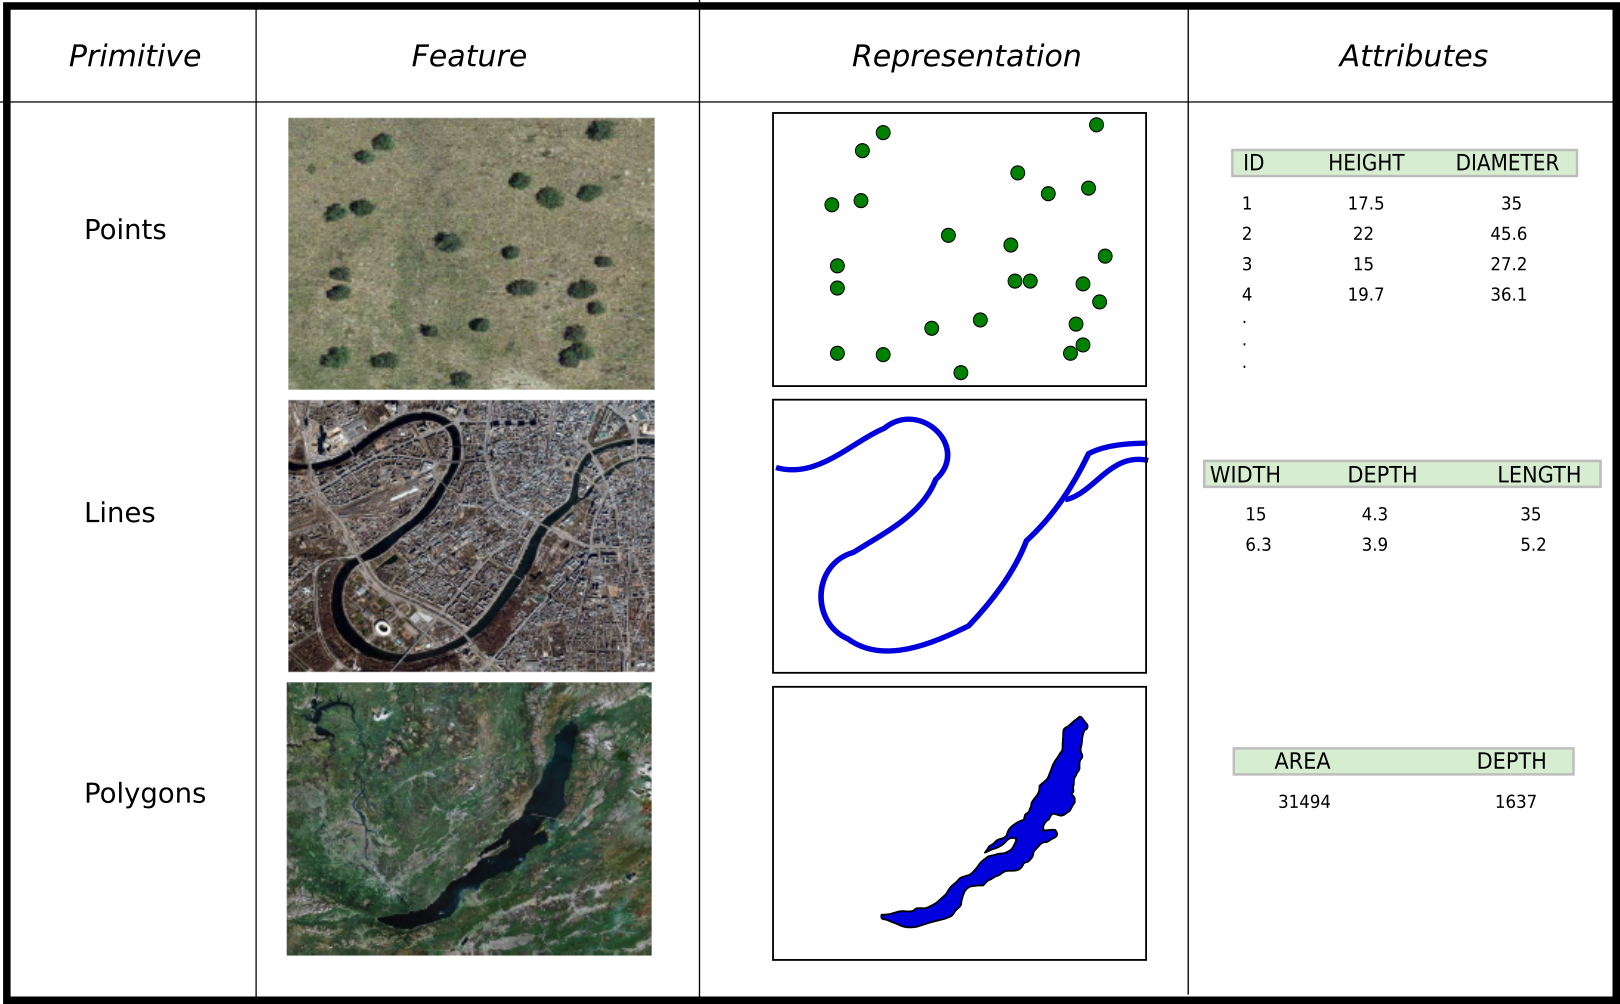
\includegraphics[width=0.8\linewidth]{obrazky-figures/geo-objects.png}
    \caption{Geografické objekty, ich reprezentácia, príklady a možné atribúty. Prevzaté z~\cite{introductiontogis}.}
    \label{fig:geo-objects}
\end{figure}

\textbf{Bod} (point) reprezentuje jednotlivý pár súradníc X, Y. Body sú bežne používané na~vizualizáciu udalostí a~javov, ktoré môžu byť identifikované špeciálnymi polohami na~mape (napr. supermarket, kostol).

\textbf{Čiara} (line) reprezentuje množinu usporiadaných bodov \--- uzlov, ktoré sú pospájané do~čiary. Tieto geometrické útvary majú jednoznačne zadefinovaný začiatočný a~koncový bod (napr. cesta, rieka).

\textbf{Polygón} (polygon) reprezentuje množinu usporiadaných bodov \--- uzlov, ktoré sú navzájom pospájané líniami do uzatvorenej plochy. Majú regionálny alebo zónový rozsah ohraničený súborom mapovateľných hraníc (napr. regióny).\\

Použitím bodov, čiar a polygónov môže byť geografický priestor modelovaný priradením hodnôt k týmto objektom. Každá časť mapy môže obsahovať viacero objektov. Napríklad pri vytváraní mapovej vrstvy s krajinami sveta by bolo potrebné, aby pre krajinu USA bolo vytvorených viacero polygónov (kontinentálna časť USA, Aljaška, Havajské ostrovy,~apod.). Všetky tieto polygóny vytvárajú jeden prvok, pretože sú súčasťou jednej krajiny a budú zdielať rovnaké priradené hodnoty~\cite{introductiontogis}.

Pri reprezentovaní špecifického prvku alebo javu na~mape nie je vždy jednoznačné, ktorý typ geografického objektu by sa mal použiť. Rovnaký geografický jav môže reprezentovať rôzne typy geografických objektov pri rôznych úrovniach priblíženia. Napríklad mesto môže byť reprezentované ako bod na~mape, ale takisto môže byť reprezentované polygónom~\cite{geographicobjects}.

% \subsection{Spracovávanie mapových dát}
% Mapové dáta, ako každé iné dáta, je možné upravovať do formy, v ktorej sú vhodnejšie na spracovávanie. 
% Geografické súradnice aj geografické objekty (ktoré sú popísané geografickými súradnicami) je možné upraviť do tvaru, ktoré môžu byť využiteľné pri dátovej analýze. Z geografických objektov je najjednoduchší na spracovanie \emph{bod}, lebo je popísaný iba dvoma hodnotami \--- zemepisnou dĺžkou a zemepisnou šírkou. Preto z~ostatných objektov je potrebné vytvoriť postupnosť bodov.



\chapter{Zdroje mapových dát}
\label{source-map-data}
Mapové dáta sa dajú získať z viacerých zdrojov. Každý takýto zdroj má svoje výhody aj nevýhody. Táto kapitola oboznámi čitateľa z akých zdrojov je možné získať mapové dáta, aké sú možné výhody a aké sú nevýhody daného zdroja, ale aj aké formáty súborov mapových dát tieto zdroje ponúkajú. 


\section{GIS}
Geografický informačný systém (GIS) je informačný systém, ktorý sa využíva na získavanie, analyzovanie, vizualizáciu a manažment dát s~priestorovým alebo mapovým vyjadrením. GIS spracováva geografické údaje v~digitálnej podobe. Časť takýchto údajov vzniká napr. pomocou satelitných údajov, meraním pomocou polohového systému GPS alebo inými meracími prístrojmi. Údaje v~papierovej podobe je nutné digitalizovať. Súčasťou GIS je hardvér (počítače, servery, zariadenia na zber dát,...), softvér (špecializované programy pre prácu s~priestorovými dátami), dáta (priestorové údaje) a~používatelia (spracovatelia dát, administrátori GIS a~prijímatelia priestorových informácií)~\cite{introductiontogis}. Používatelia systému môžu využívať rôzne metódy spracovania geografických údajov, ktoré umožňujú údaje prehľadávať, triediť, reklasifikovať, transformovať a~modelovať~\cite{hofierka2003gis}.

Geografické dáta v GIS môžu byť organizované dvomi základnými modelmi \--- vektorovým a rastrovým modelom~\cite{holman2014priestorovedata}.

\subsection{Vektorový model}
Vektorový model je nazývaný podľa spôsobu vyjadrenia jeho jednotlivých častí \--- úseky kriviek s definovanou veľkosťou a smerom \--- \emph{vektorom}. Vektorový model GIS pracuje s~tromi variantami geografických objektov \--- bod, čiara a polygón.

Existujú rôzne modely dát pomocou ktorých je možné reprezentovať geografické objekty s~využitím vektorovej grafiky:
\begin{itemize}
    \item \textbf{Špagetový model} \--- vychádza z postupov využívaných pri digitalizácií máp. Každý objekt na mape je reprezentovaný jedným záznamom a je uložený ako reťazec X, Y súradníc. Z tohto modelu nie je možné získať žiadne informácie o vzťahoch medzi jednotlivými subjektami aj keď sa jedná o priestorové dáta.
    \item \textbf{Topologický model} \--- každá línia tohto modelu začína a končí v uzlu. Všetky informácie tohto modelu sú ukladané do tzv. \emph{topologických tabuliek} \--- tabuľka spojov, súradníc a polygónov. Model vďaka tomu uchováva priestorové vzťahy medzi objektami.
    \item \textbf{Hierarchický model} \--- ukladá zvlášť informáciu o bodoch, líniách a plochách v~hierarchickej štruktúre pre jednoduchšie vyhľadávanie v dátach. V modeli sú takisto zahrnuté aj odkazy medzi jednotlivými druhmi objektov a obsahuje topologickú informáciu. Tento model je pre manipuláciu a vyhľadávanie v dátach najvhodnejší.
\end{itemize}

\subsubsection{Vektorové formáty dát}
Medzi najznámejšie vektorové formáty dát patrí formát \emph{shapefile} vytvorený spoločnosťou ESRI. Tento formát sa ukladá do zariadenia ako skupina aspoň troch súborov, ktoré síce majú rovnaký názov, ale majú rôznu príponu:
\begin{itemize}
    \item hlavný súbor \texttt{*.shp} \--- obsahuje popis geometrie každého záznamu
    \item indexový súbor \texttt{*.shx} \--- prepája prvok v hlavnom súbore so záznamom v atribútovej tabuľke
    \item databázový súbor \texttt{*.dbf} \--- databázový súbor, obsahuje dáta atribútov pre každý záznam
\end{itemize}

Okrem hore zmienených súboroch môže mať \emph{shapefile} aj iné súbory, ktoré obsahujú ďalšie informácie o dátach:
\begin{itemize}
    \item projekčný súbor \texttt{*.prj} \--- ukladá informácie o súradnicovom systéme
    \item priestorové indexy \texttt{*.gix}, \texttt{*.sbn}, \texttt{*.sbx} \--- umožňujú rýchlejšie vyhľadávanie prvkov
    \item atribútové indexy \texttt{*.atx} \--- urýchľujú vyhľadávanie v atribútovej tabuľke
    \item metadátový súbor \texttt{*.shp.xml} \--- metadáta o zvolenom prvku
    \item kódovací súbor \texttt{*.cpg} \--- súbor pre správnu identifikáciu znakov
\end{itemize}

Existuje veľa iných vektorových formátov dát, ktoré sa používajú v GIS ako napr. \emph{KML}, \emph{KMZ}, \emph{GPX} a \emph{GeoJSON}

\textbf{KML} (Keyhole Markup Language) je dátový formát vyvinutý pre aplikáciu Google Earth. Okrem ukladania informácií o geometrii obsahuje možnosti konfigurácie pre Google Earth mapy.

\textbf{KMZ} (Keyhole Markup Zipped) je dátový formát, ktorý sa takisto používa v aplikáciách Google. Tento formát je rozšírením KML formátu, pretože obsahuje okrem textového popisu aj obrázky tvoriace 3D vizualizácie prvku.

\textbf{GPX} (GPS Exchange Format) je formát údajov GPS pre ukladanie bodov, trás a ich atribútov. Ukladá informácie pomocou textu, podobne ako súbory typu KML.

\textbf{GeoJSON}~\cite{rfc7946} je formát založený na formáte JSON (Javascript Object Notation\footnote{\url{https://www.json.org}}). Tento formát je navrhnutý pre reprezentáciu jednoduchých priestorových geografických dát a ich atribútov. Pomocou tohto formátu je možné reprezentovať nasledujúce geometrické typy: \emph{Point}, \emph{LineString}, \emph{Polygon}, \emph{MultiPoint}, \emph{MultiLineString} a \emph{MultiPolygon}. Vo výpise~\ref{lst:geojson} je možné vidieť, ako je reprezentovaný bod (Point) vo formáte GeoJSON.

\lstset{
    caption={\texttt{FeatureCollection} obsahuje vo vlastnosti \texttt{features} objekt typu \texttt{Feature}, ktorý v \texttt{properties} obsahuje informácie viazané na objekt \texttt{geometry}.},
    label={lst:geojson},
    basicstyle=\ttfamily\footnotesize\bfseries,
    xleftmargin=.2\textwidth, xrightmargin=.2\textwidth
}
\begin{lstlisting}
{
  "type": "FeatureCollection",
  "features": [
    {
      "type": "Feature",
      "properties": {
        "kraj": "Moravsko-sliezsky",
      },
      "geometry": {
        "type": "Point",
        "coordinates": [
          17.60100156068802,
          49.196293610455584
        ]
      }
    }
  ]
}
\end{lstlisting}

\subsection{Rastrový model}
Rastrová reprezentácia mapových dát sa na rozdiel od vektorovej zameriava na zemský povrch. Používa sa skôr na javy ako je napr. úhrn zrážok či nadmorská výška.

Základným princípom tohto formátu je pokrytie zemského povrchu pravidelnou alebo nepravidelnou sieťou, pričom jednotka tieto siete je \emph{bunka} (pixel, cell). Nepravidelná sieť má výhodu oproti nepravidelnej siete takú, že pomocou nepravidelnej siete je možné jednoduchšie reprezentovať rôzne prechody z roviny na terénnu hranu. Na druhú stranu použitie nepravidelnej siete je výpočtovo a aj algoritmicky náročnejšie. Keďže v tomto modeli neexistujú objekty známe z vektorového modelu GIS, bunky definujú vlastnú hodnotu sledovaného javu v konkrétnej časti priestoru. Hodnota v jednej bunke odpovedá bodu, rada spojených buniek s rovnakou hodnotou odpovedá línii a skupina navzájom susediacich buniek odpovedá ploche.

\begin{figure}[ht]
    \centering
    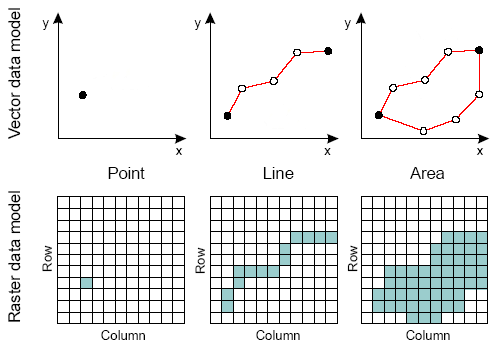
\includegraphics[width=0.5\linewidth]{obrazky-figures/vector-and-raster-data.png}
    \caption{\textbf{Vektorový a rastrový dátový model}. Prevzaté z~\cite{jukil2017mapdata}.}
    \label{fig:vectorandraster}
\end{figure}

\subsection{ArcGIS}
V súčasnosti existujú rôznorodé softvéry pre GIS. Medzi najznámejšie patrí ArcGIS od~spoločnosti ESRI, ktorý slúži na mapovanie a priestorovú analýzu navrhnutý tak, aby podporoval poslanie a obchodné ciele organizácií. Tento systém poskytuje tri úrovne licencií. Typ zvolenej licencie rozhoduje o tom, ako sú uložené dáta a ako je možné ich editovať. 

Medzi najznámejšie aplikácie systému ArcGIS patrí ArcMap (použiteľná na priestorové analýzy, editáciu dát a tvorbu kartografických výstupov), ArcCatalog (pomáha organizovať a spravovať všetky dáta), ArcGIS Explorer (volne dostupný prehliadač priestorových dát), ArcGIS for~Server (serverové riešenie pre GIS, umožňuje jednoduchú konfiguráciu webových aplikácií a poskytuje kompletné vývojárske prostredie pre \emph{.NET} a \emph{Java}).

\subsection{ArcČR 500}
ArcČR 500~\cite{arcgis} je digitálna vektorová geografická databáza Českej republiky, spracovaná na úrovni podrobnosti 1 : \numprint{500000}. Obsahom databázy sú prehľadné geografické informácie o~ČR. Zdrojom dát pre geografické dáta ArcČR 500 v 3.3 je databáza Data200, čo je národná vektorová geografická databáza Zeměměřického úřadu (ZÚ) odpovedajúca presnosťou a~stupňom generalizácie 1 : \numprint{200000}. Vstupné dáta z Data200 majú deklarovanú absolútnu presnosť do 100 m. Absolútna polohová odchýlka ArcČR 500 v 3.3 je odhadovaná do 200~m.

Dáta sú uchovávané iba v GIS formátoch firmy ESRI a to vo formáte súborovej databázy. ArcČR 500 je zložená z dvoch geodatabází \--- geografické prvky a administratívne členenie.

\subsubsection*{Geografické prvky}
Geografické prvky boli odvodené zo 17-tich vrstiev databázy Data200. Vrstvy súborovej databázy \texttt{ArcCR500\_v33.gdb} ako aj ich popis a typ prvkov je možné vidieť v tabuľke~\ref{tab:arccr500}.

\begin{table}[H]
\begin{tabular}{|l|p{0.5\linewidth}|l|}
    \hline
    \textbf{vrstva}        & \textbf{popis}                                 & \textbf{typ prvku} \\ \hline
    Letiste                & Letisko                                        & bod                \\
    SidlaBody              & Sídla nad 500 obyvateľov                       & bod                \\
    VyskoveKoty            & Výškové kóty (vrcholy kopcov)                  & bod                \\
    ZeleznicniStanice      & Železničná stanica                             & bod                \\
    Hranice                & Štátna, krajská a okresná hranica              & línia              \\
    Silnice                & Cesta                                          & línia              \\
    VodniToky              & Vodné toky                                     & línia              \\
    Vrstevnice             & Vrstevnice po 25 m                             & línia              \\
    Zeleznice              & Železnice                                      & línia              \\
    BazinyARaseliniste     & Močiar a rašelinisko väčšie ako 30 ha          & polygón            \\
    Lesy                   & Lesné plochy väčšie ako 30 ha                  & polygón            \\
    SidlaPlochy            & Sídla nad \numprint{5000} obyvateľov           & polygón            \\
    VodniPlochy            & Vodné plochy väčšie ako 15 ha                  & polygón            \\
    ChranenaUzemi          & Národné parky a chránené krajinné oblasti      & polygón            \\
    KladyZakladnichMap     & Klady základných máp ČR                        & polygón            \\
    KladyTopografickychMap & Klady vojenských topografických máp            & polygón            \\
    SouradnicovaSitJTSK    & Súradnicová sieť systému JTSK v intervale 1~km & línia              \\
    ZemepisnaSitETRS89     & Zemepisná sieť v systéme ETR89                 & línia              \\
    ZemepisnaSitWGS84      & Zemepisná sieť v systéme WGS84                 & línia              \\
    DigitalniModelReliefu  & Raster digitálneho modelu reliéfu              & raster             \\
    StinovanyRelief        & Raster tieňovaného modelu reliéfu              & raster             \\ \hline
\end{tabular}
\caption{Súborová databáza ArcCR500\_v33.gdb. Prevzaté z~\cite{arcgis}.}
\label{tab:arccr500}
\end{table}

Každá vrstva tejto databázy môže nadobúdať rôzne hodnoty atribútov, ktoré sú pre danú vrstvu zadefinované. V tejto práci sú uvedené pre ilustráciu iba vrstvy Letisko (tabuľka~\ref{tab:letisko}) a Hranica (tabuľka~\ref{tab:hranica}). V tabuľke \ref{tab:letisko} je možné vidieť, že atribút \texttt{TYP} môže nadobúdať tri hodnoty \--- t.j.~letisko je buď civilné alebo vojenské, alebo civilné a vojenské. Táto vrstva je zobrazená na mape ako bod. Na druhú stranu vrstva \emph{Hranica}, ktorá sa zobrazuje na mape ako línia, nemá takú variabilitu atribútov ako vrstva \emph{Letisko}. V tabuľke~\ref{tab:hranica} je možné vidieť, že daná vrstva má iba jeden zadefinovaný atribút, ktorý ale môže nadobúdať 3 hodnoty \--- t.j. hranica môže byť štátna, krajská alebo okresná.

\begin{table}[H]
    \centering
    \begin{tabular}{|l|l|l|}
    \hline
    \textbf{meno atribútu}         & \textbf{popis}      & \textbf{nadobúdané hodnoty}   \\ \hline
    \textbf{TYP}          & Typ letiska         & \begin{tabular}[c]{@{}l@{}}1 - civilné\\ 2 - vojenské\\ 3 - civilné a vojenské\end{tabular} \\
    \textbf{NAZEV}        & Meno                & \textit{konkrétne meno}       \\
    \textbf{NAZEV\_ASCII} & Meno (ASCII formát) & \textit{konkrétne meno}       \\
    \textbf{ICAO}         & Kód ICAO            & \textit{konkrétny kód}        \\
    \textbf{STATUT}       & Statut letiska      & \begin{tabular}[c]{@{}l@{}}1 - medzinárodné\\ 2 - vnútroštátne\end{tabular}                 \\ \hline
    \end{tabular}
\caption{Vrstva Letisko (Letiste). Prevzaté z~\cite{arcgis}.}
\label{tab:letisko}
\end{table}

\begin{table}[H]
    \centering
    \begin{tabular}{|l|l|l|}
        \hline
        \textbf{meno atribútu} & \textbf{popis} & \textbf{nadobúdané hodnoty}  \\ \hline
        \textbf{TYP}  & Typ hranice    & \begin{tabular}[c]{@{}l@{}}1 - štátna\\ 2 - krajská\\ 3 - okresná\end{tabular} \\ \hline
    \end{tabular}
    \caption{Vrstva Hranica (Hranice). Prevzaté z~\cite{arcgis}.}
    \label{tab:hranica}
\end{table}

\subsubsection*{Administratívne členenie}
Dáta z Českého statistického úřadu (ČSÚ) boli použité pre tvorbu dát administratívneho členenia. Vrstvy súborovej geodatabázy \texttt{AdministrativniCleneni\_v13.gdb} ako aj ich popis sa nachádza v tabuľke~\ref{tab:administrativne-clenenie}.
\begin{table}[H]
    \centering
    \begin{tabular}{|lll|}
    \hline
    \textbf{názov}  & \textbf{popis}                 & \textbf{typ prvku} \\ \hline
    \textbf{ZSJ}    & Základné sídelné jednotky      & bod/polygón        \\
    \textbf{UTJ}    & Územné technické jednotky      & bod/polygón        \\
    \textbf{KU}     & Katastrálne územie             & bod/polygón        \\
    \textbf{MOaMC}  & Mestské obvody a mestské časti & bod/polygón        \\
    \textbf{COB}    & Časti obce                     & bod/polygón        \\
    \textbf{OBCE}   & Obce a vojenské újazdy         & bod/polygón        \\
    \textbf{POU}    & Obce s povereným úradom        & bod/polygón        \\
    \textbf{ORP}    & Obce s rozšírenou pôsobnosťou  & bod/polygón        \\
    \textbf{OKRESY} & Okresy                         & bod/polygón        \\
    \textbf{KRAJE}  & Kraje                          & bod/polygón        \\
    \textbf{STAT}   & Štát                           & bod/polygón        \\ \hline
    \end{tabular}
    \caption{Súborová databáza AdministrativniCleneni\_v13.gdb. Prevzaté z~\cite{arcgis}.}
    \label{tab:administrativne-clenenie}
\end{table}


\section{OpenStreetMap}
OpenStreetMap~\cite{openstreet} je projekt, ktorý vznikol za účelom vytvárania geografickej databázy celého sveta. Cieľom tohto projektu je mať časom záznam o každom geografickom prvku na~planéte. Zatiaľ čo to začalo mapovaním ulíc, postupom času tento projekt zahŕňa chodníky, budovy, vodné cesty, potrubia, lesy, pláže, poštové schránky a dokonca aj jednotlivé stromy.

\subsection{História projektu}
Projekt OpenStreetMap má svoj začiatok v auguste v roku 2004, kedy britský programátor Steve Coast experimentoval s USB GPS prijímačom. Použil softvér nazývaný GPSDrive, ktorý bral mapy z Microsoft MapPoint, ale porušoval licenčné podmienky. Coast vedome nechcel porušovať autorské práva týchto máp, preto hľadal alternatívu, ktorá by neporušovala licenčné podmienky, tú ale nenašiel. Zistil, že neexistujú zdroje mapových dát, ktoré by mohol používať v otvorenom softvére bez toho, aby porušoval licenčné podmienky alebo platil obrovské sumy peňazí. Po odprezentovaní jeho nápadu o vytvorení vlastnej mapy na konferencii otvorených softvérov v Londýne zistil, že viacerí ľudia mali podobný nápad alebo ich Coastov nápad zaujal, a tak vznikla skupina OpenStreetMap.

V začiatkoch bol dátový model príliš simplistický, pretože obsahoval iba jednoduché čiary nakreslené cez informácie Landsat od NASA. V marci v roku 2006 bola vytvorená prvá editovacia aplikácia pre OpenStreetMap \--- JOSM\footnote{\url{https://josm.openstreetmap.de/}}. Po chvíli bola v tomto roku vytvorená prvá plnofarebná mapa mesta Weybridge. V máji toho roku sa usporiadala prvá spoločná akcia, na ktorej bolo úlohou zmapovať ostrov Wight. Bolo to prvýkrát, kedy sa stretlo viacero mapovačov a znamenalo to pre nich prelomový bod projektu, pretože bola vytvorená detailná mapa. Takéto akcie OpenStreetMap komunity sa začali konať častejšie a boli usporadúvané po celom svete.

V auguste v roku 2006 bola vytvorená nadácia \emph{OpenStreetMap Foundation}, ktorou úlohu je podporovať, ale nie kontrolovať OpenStreetMap projekt. Venuje sa podpore rastu, rozvoja a distribúcii voľne dostupných geografických dát a poskytovaniu geografických údajov komukoľvek na používanie a zdieľanie.

Serverový softvér bol pôvodne napísaný v programovacom jazyku Java, ale v~máji v~roku 2007 bola implementácia softvéru prepísaná do platformy Ruby on Rails\footnote{\url{https://rubyonrails.org/}}. Časom ako začal projekt postupne narastať, začali svojimi dátami prispievať súkromné spoločnosti, mestá, ale aj štáty~\cite{bennett2010openstreetmap}. Vo februári v roku 2008 bolo zaregistrovaných \numprint{25000} užívateľov na~stránke OpenStreetMap, v marci v roku 2009 to už bolo \numprint{100000} užívateľov. Počet užívateľov stále rastie, v čase písanie tohto textu je to už viac ako 8,3 milióna zaregistrovaných užívateľov.

\begin{figure}[ht]
    \centering
    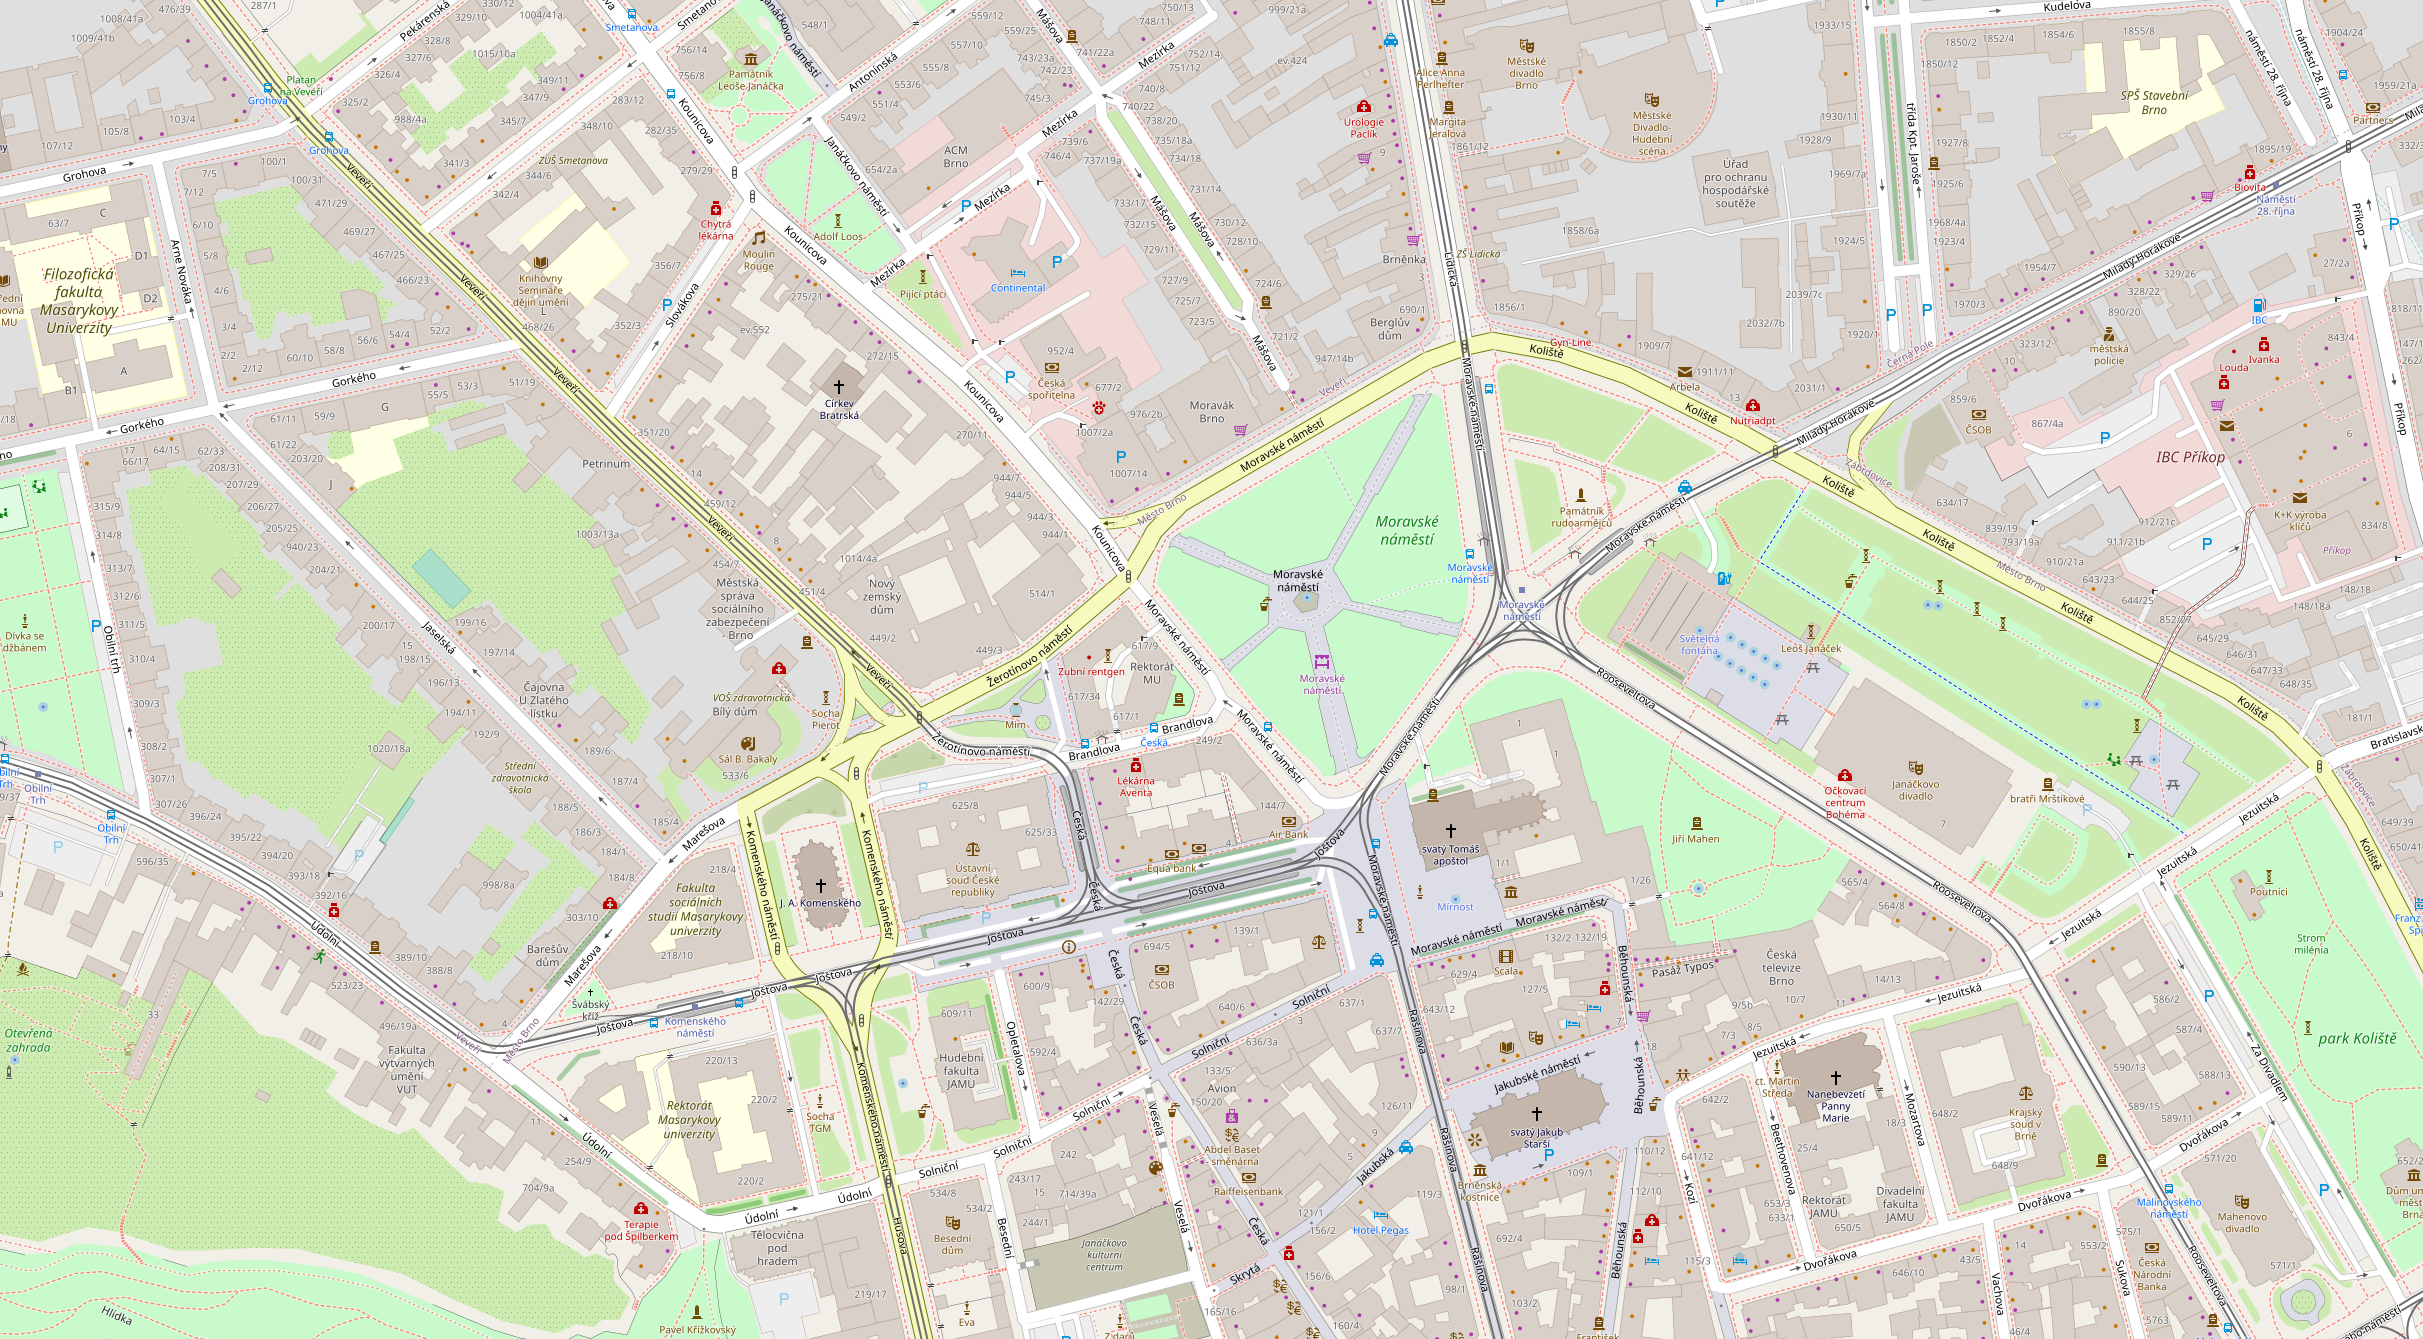
\includegraphics[width=\linewidth]{obrazky-figures/openstreetmap.png}
    \caption{\textbf{OpenStreetMap}. Výsek z mapy časti Brna.}
    \label{fig:openstreetmap}
\end{figure}

\subsection{Dátový model OpenStreetMap}
Prvky (anglicky elements) sú základnou stavebnou súčasťou dátového modelu OpenStreetMap slúžiace k popisu reálneho sveta. Medzi základné prvky OpenStreetMap projektu patria uzol, cesta a relácia. Tieto prvky je možné popísať značkami.

\textbf{Uzol\footnote{\url{https://wiki.openstreetmap.org/wiki/Node}}} (anglicky node) označuje konkrétny bod na povrchu Zeme, je určený svojou zemepisnou šírkou a dĺžkou. Skladá sa minimálne z dvojice súradníc a svojho jednoznačného identifikačného čísla (id).

\textbf{Cesta\footnote{\url{https://wiki.openstreetmap.org/wiki/Way}}} (anglicky way) je usporiadaný zoznam 2 až \numprint{2000} uzlov, ktoré definujú lomenú čiaru. Cesta má aspoň jednu značku alebo je vložená do relácie.

\textbf{Relácia\footnote{\url{https://wiki.openstreetmap.org/wiki/Relation}}} (anglicky relation) sa skladá z jednej alebo viacerých značiek a usporiadaného zoznamu jedného alebo viacerých uzlov alebo ciest. Každý prvok relácie je tzv. člen (anglicky member). Používa sa k popisu závislosti medzi rôznymi prvkami. Každý člen relácie môže voliteľne mať nejakú rolu, ktorá popisuje jeho význam v rámci relácie.

\textbf{Značka\footnote{\url{https://wiki.openstreetmap.org/wiki/Tags}}} (anglicky tag) sa skladá z kľúča a hodnoty. Každá značka popisuje určitú vlastnosť dátových prvkov (uzlov, ciest a relácií) alebo sadu zmien. Kľúč popisuje tému, kategóriu alebo typ mapového prvku (napr. cesta \--- \emph{highway} alebo názvy \--- \emph{name}). Hodnota konkretizuje vlastnosť, ktorú všeobecne popisuje kľúč. Napríklad značka \texttt{highway=residential} predstavuje cestu, ktorá vedie obytnou oblasťou.

\begin{figure}[ht]
    \centering
    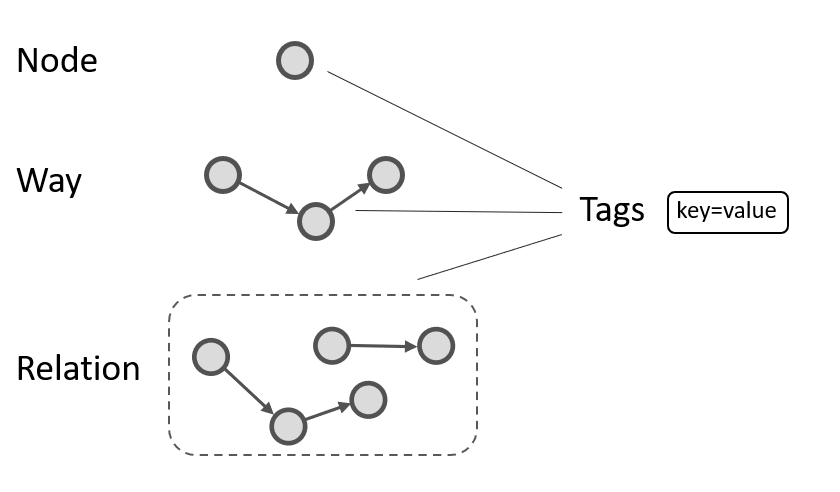
\includegraphics[width=0.64\linewidth]{obrazky-figures/openstreetmap-datamodel.png}
    \caption{\textbf{Dátový model OpenStreetMap}. Prevzaté z~\cite{jafari2022building}.}
    \label{fig:osmdatamodel}
\end{figure}


\section{Kataster}
Kataster predstavuje register resp. zoznam a používa sa vo viacerých významoch:
\begin{itemize}
    \item súpis nehnuteľného majetku, ktorý bol vytvorený pre daňové a úradné účely
    \item kataster nehnuteľností, katastrálna kniha
    \item katastrálne územie
\end{itemize}

\subsection{Kataster nehnuteľností}
Súčasný kataster nehnuteľností~\cite{baudys-katastranemovitosti} na území Českej republiky mal ekvivalent medzi svojimi právnymi predchodcami \--- tzv.~pozemkovú knihu, ktorá slúžila na majetkoprávne účely. Okrem pozemkovej knihy sa používal aj pozemkový kataster, ktorý slúžil na~daňové účely. Pozemkový kataster sa používal približne do roku 1957 a zapisovanie do~pozemkovej knihy bol ukončený v~roku 1964, pretože nevypovedala o~skutočných a~aktuálnych právnych vzťahoch k~nehnuteľnostiam. Preto bola vytvorená nová pozemková evidencia nehnuteľností, ktorej hlavným účelom bolo zaistiť podklady pre plánovanie národného hospodárstva. Táto evidencia bola vedená až do roku 1992, kedy si spoločenské zmeny vyžiadali založenie dnešného katastru nehnuteľností.

Dnešný kataster nehnuteľností plní úlohu pozemkovej knihy aj pozemkového katastru a slúži aj ako podklad pre geografické informačné systémy. Kataster nehnuteľností je definovaný ako súbor údajov o nehnuteľností v Českej republike. Okrem súpisu a popisu nehnuteľností zahŕňa ich geometrické a polohové určenie pre jednu katastrálnu obec alebo katastrálne územie. Aj keď v českom katastri sú zapísané všetky pozemky, zo stavieb sú zapísané v katastri len tie budovy, ktoré stanovuje katastrálny zákon. Ide o budovy s popisným či evidenčným číslom alebo hlavnú budovu v rámci areálu nehnuteľností. Na obrázku~\ref{fig:katastrmapa} je možné vidieť ako vyzerá katastrálna mapa mestskej časti Brno-Královo Pole. Obrázok je exportovaný zo stránky Českého katastru nemovitostí\footnote{\url{https://nahlizenidokn.cuzk.cz/VyberKatastrMapa.aspx}}, ktorý okrem faktických a právnych informácií o nehnuteľnostiach obsahuje katastrálne mapy a informácie o vlastníkoch nehnuteľností.

\begin{figure}[ht]
    \centering
    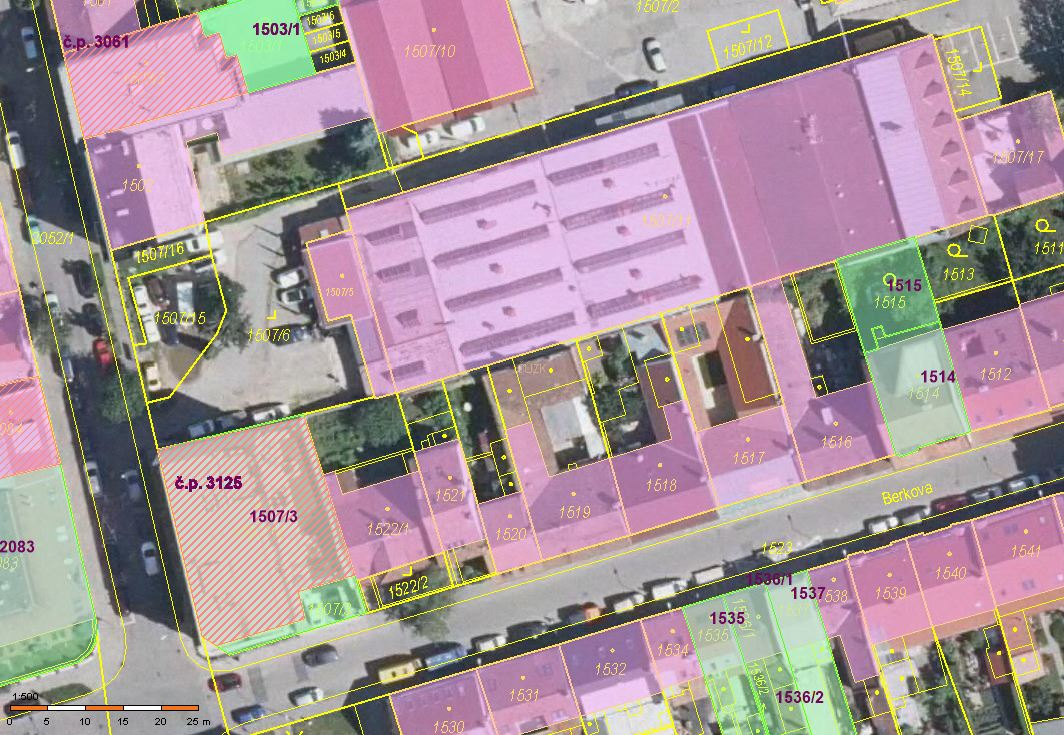
\includegraphics[width=0.8\textwidth]{obrazky-figures/katastr-ortofo-kralovopole.jpg}
    \caption{\textbf{Katastrálna mapa s ortofotomapou mestskej časti Brno-Královo Pole}. Ružová farba predstavuje budovy, budovy so zelenou farbou sú nehnuteľnosti s~cenovými údajmi k~jednotke (byty alebo nebytové priestory), vyšrafované budovy sú nehnuteľnosti s~cenovými údajmi k~parcele.}
    \label{fig:katastrmapa}
\end{figure}

\subsection{Územný plán}
Vlastníci katastrov nehnuteľností si musia byť istý, že na danom území existuje poriadok, ktorý by mal zaručovať, že ich práva nebudú ohrozované náhodnými a~meniacimi sa rozhodnutiami. Územným plánovaním sa predchádza nekoncepčnému a zložitému rozvoja obce. Zaoberá sa všetkými aspektmi nášho prostredia. Ide prevažne o~stavbu sídiel, dopravnú a~ technickú infraštruktúru, ale aj o prvky, ktoré vytvárajú prírodné zložky životného prostredia~\cite{uzemnyplan}.



\chapter{Využité technológie}
\label{technology}
V tejto kapitole sú preberané všetky technológie, ktoré boli použité pri vytváraní užívateľského rozhrania. Ku každej technológií sú napísané dôvody, prečo bola zvolená technológia vhodná na použitie. Aplikácia bola navrhnutá ako klient-server aplikácia, t.j. na strane klienta bolo použité technológie na vizualizáciu výstupov a~na~strane serveru technológie na~spracovávanie dát poslaných od klienta.


\section{GeoPandas}
GeoPandas\footnote{\url{https://geopandas.org/en/stable}} je open-source projekt, ktorý umožňuje jednoduchú manipuláciu geografických dát v jazyku Python. Tento projekt je pokročilejší nástroj umožňujúci načítavanie GIS dát (.geojson, .gdb, .shp, \ldots), manipuláciu s GIS dátami, manipuláciu s~geometrickými útvarmi, prevádzanie súradnicových systémov a vykresľovanie máp. Základnými dátovými štruktúrami projektu GeoPandas sú \texttt{GeoDataFrame} a \texttt{GeoSeries}. Tieto dve dátové štruktúry sú nadstavbou knižnice \emph{Pandas}\footnote{\url{https://pandas.pydata.org}}, pretože rozširujú možnosti dátových štruktúr \texttt{Series} a \texttt{DataFrame} z tejto knižnice. Táto aplikácia je esenciálnou súčasťou celej aplikácie, pretože ju používajú aj iné knižnice.

\texttt{GeoDataFrame} je dvojrozmerná dátová štruktúra, podobná tabuľke s riadkami a~stĺpcami a~je podtriedou \emph{pandas.DataFrame} s pridaným stĺpcom \texttt{geometry} (obrázok~\ref{fig:dataframes}).

\texttt{GeoSeries} je jednorozmerná dátová štruktúra, ktorá je podtriedou \emph{pandas.Series} a~umožňuje ukladať geometrické objekty \--- body, čiary, polygóny, prípadne ich násobné varianty. Predstavuje stĺpec geometry v dátovej štruktúre GeoDataFrame.

\begin{figure}[ht]
    \centering
    \subfloat[\centering \textbf{DataFrame}]{{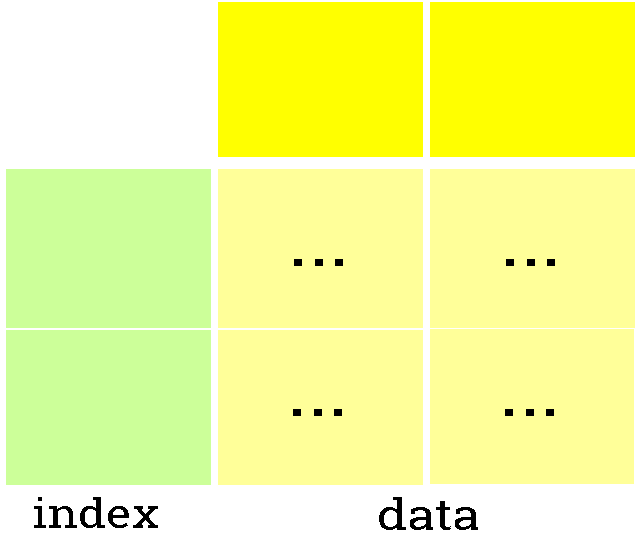
\includegraphics[width=0.25\linewidth]{obrazky-figures/dataframe.pdf}}}
    \qquad
    \subfloat[\centering \textbf{GeoDataFrame}]{{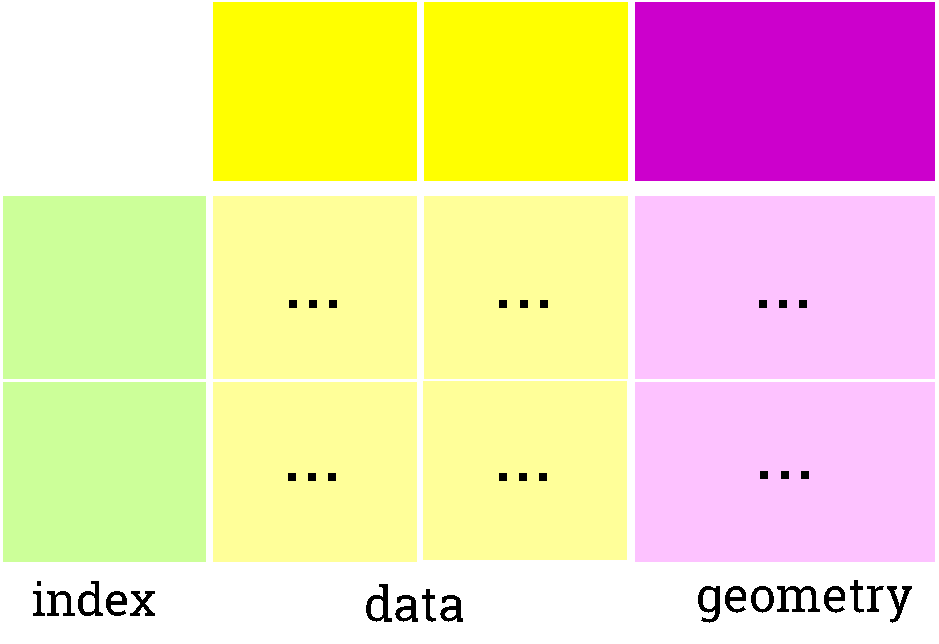
\includegraphics[width=0.31\linewidth]{obrazky-figures/geodataframe.pdf}}}
    \caption{Rozdiel medzi dátovými štruktúrami DataFrame a GeoDataFrame.}
    \label{fig:dataframes}
\end{figure}


\section{OSMnx}
Aby bolo možné pracovať s geografickými dátami, je potrebné ich stiahnuť z určitého zdroja. V~jazyku Python existuje balíček OSMnx\footnote{\url{https://osmnx.readthedocs.io/en/stable}}, ktorý umožňuje sťahovať geopriestorové dáta z~OpenStreetMap. Okrem sťahovania umožňuje tento balíček modelovať, projektovať, zobrazovať a analyzovať pouličné siete reálneho sveta. Balíček OSMnx obsahuje viacero modulov, na túto prácu bol potrebný iba jeden modul \--- modul \texttt{geometries}, ktorý  umožňuje sťahovanie geopriestorových atribútov a entít z OpenStreetMap. Modul sťahuje dáta z OpenStreetMap Nominatim API\footnote{\url{https://nominatim.org}} a vracia dátovú štruktúru GeoDataFrame.


\section{Flask}
Flask\footnote{\url{https://flask.palletsprojects.com/en/2.1.x}} je mikro webový framework napísaný v programovacom jazyku Python. Flask nevyžaduje konkrétne nástroje ani ďalšie vnútorné knižnice. Aj keď sa tento framework považuje za mikro framework, neznamená to, že nie je možné ho rozširovať o rôzne služby~\cite{Oreilly2014Flask}.

Flask som si vybral kvôli jeho jednoduchosti a kvôli tomu, že navrhnutá aplikácia nevyžaduje na prevádzku integráciu s databázovou schémou, ktorú treba integrovať u iných webových frameworkoch. Navyše navrhnutá aplikácia je iba jednostránková aplikácia, takže využívanie robustných webových frameworkov by bolo nepraktické.


\section{Leaflet}
Leaflet\footnote{\url{https://leafletjs.com}} je open-source knižnica v programovacom jazyku JavaScript, používaná na vytváranie mapových webových aplikácii. Táto knižnica je podporovaná na väčšine mobilných a desktopových zariadeniach. Leaflet umožňuje vývojárom jednoducho zobrazovať webové mapy s dlaždicami, získať geopriestorové dáta zo súborov typu GeoJSON, vytvárať interaktívne vrstvy apod.

\subsection{Rozšírenia knižnice}
Okrem základnej funkcionality existujú rôzne rozšírenia, ktoré rozširujú základnú funkcionalitu knižnice Leaflet. V mojej aplikácii sa používajú dve rozšírenia k tejto knižnici: \texttt{Leaflet.heat} a~\texttt{Leaflet.draw}. 

\subsubsection{Rozšírenie Leaflet.heat}
Základom tejto knižnice je knižnica \texttt{simpleheat} z jazyka JavaScript, ktorá sa používa na kreslenie heat máp na plátno. Na vytvorenie vrstvy heat mapy sa používa funkcia \texttt{L.heatLayer(latlngs, options)}, kde:
\begin{itemize}
    \item \texttt{latlngs} \--- predstavuje dvojrozmerné pole, kde každé pole v tomto poli je definované dvojicou (zemepisná dĺžka, zemepisná šírka) resp. trojicou hodnôt (zemepisná dĺžka, zemepisná šírka, intenzita),
    \item \texttt{options} \--- má viacero možnosti, ktoré sa dajú zadefinovať pre danú vrstvu, najdôležitejšie z nich pre moju aplikáciu sú:
    \begin{itemize}
        \item \texttt{max} \--- maximálna intenzita bodu, implicitná hodnota je 1.0
        \item \texttt{radius} \--- rádius každého bodu na heat mape, implicitná hodnota je 25
        \item \texttt{blur} \--- množstvo rozptýlenia, implicitná hodnota je 15
        \item \texttt{gradient} \--- konfigurácia prechodu farieb
    \end{itemize}
\end{itemize}
Na~obrázku~\ref{fig:leafletheat} je možné vidieť ako sa dá pridať tepelná vrstva do mapy a ako daná vrstva vyzerá na mape.

\lstset{
    caption={},
    label={},
    basicstyle=\ttfamily\footnotesize\bfseries
}
\begin{figure}[ht]
\begin{minipage}{.5\textwidth}
\begin{lstlisting}
var heat = L.heatLayer([
     // lat, lng, intensity
    [49.1784, 16.7772, 0.2],
    [49.1784, 16.7774, 0.4],
    [49.1784, 16.7776, 0.6],
    [49.1784, 16.7778, 0.8],
    [49.1784, 16.7780, 1.0]
], {radius: 30}).addTo(map);
\end{lstlisting}
\end{minipage}
\hfill
\begin{minipage}{.5\linewidth}
    \centering
    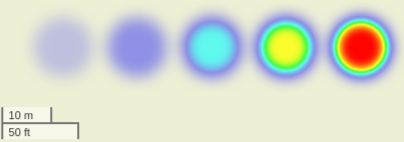
\includegraphics[width=0.7\linewidth]{obrazky-figures/heatlayer-screenshot.png}
\end{minipage}
\caption{\textbf{Rozšírenie Leaflet.heat}. Vľavo sa nachádza implementácia vrstvy, zoradená vzostupne podľa hodnôt intenzít, vpravo sa nachádza zobrazenie týchto bodov na~mape.}
\label{fig:leafletheat}
\end{figure}

\subsubsection{Rozšírenie Leaflet.draw}
Na to, aby užívateľ mohol vybrať určitú oblasť z mapy, na ktorej sa má vykresliť vrstva heat mapy, bolo potrebné použiť rozšírenie Leaflet.draw. Ako je možné vidieť na obrázku~\ref{fig:leafletdraw}, na bočnom paneli mapy v hornom ľavom rohu sa nachádza panel nástrojov, ktorý umožňuje kresliť geometrické útvary na mapu a následne ich upravovať alebo aj vymazávať. Pre~jednoduchosť aplikácie na vybratie určitej oblasti pomocou geometrických tvarov bol použitý iba jeden geometrický tvar \--- obdĺžnik.

\begin{figure}[ht]
    \centering
    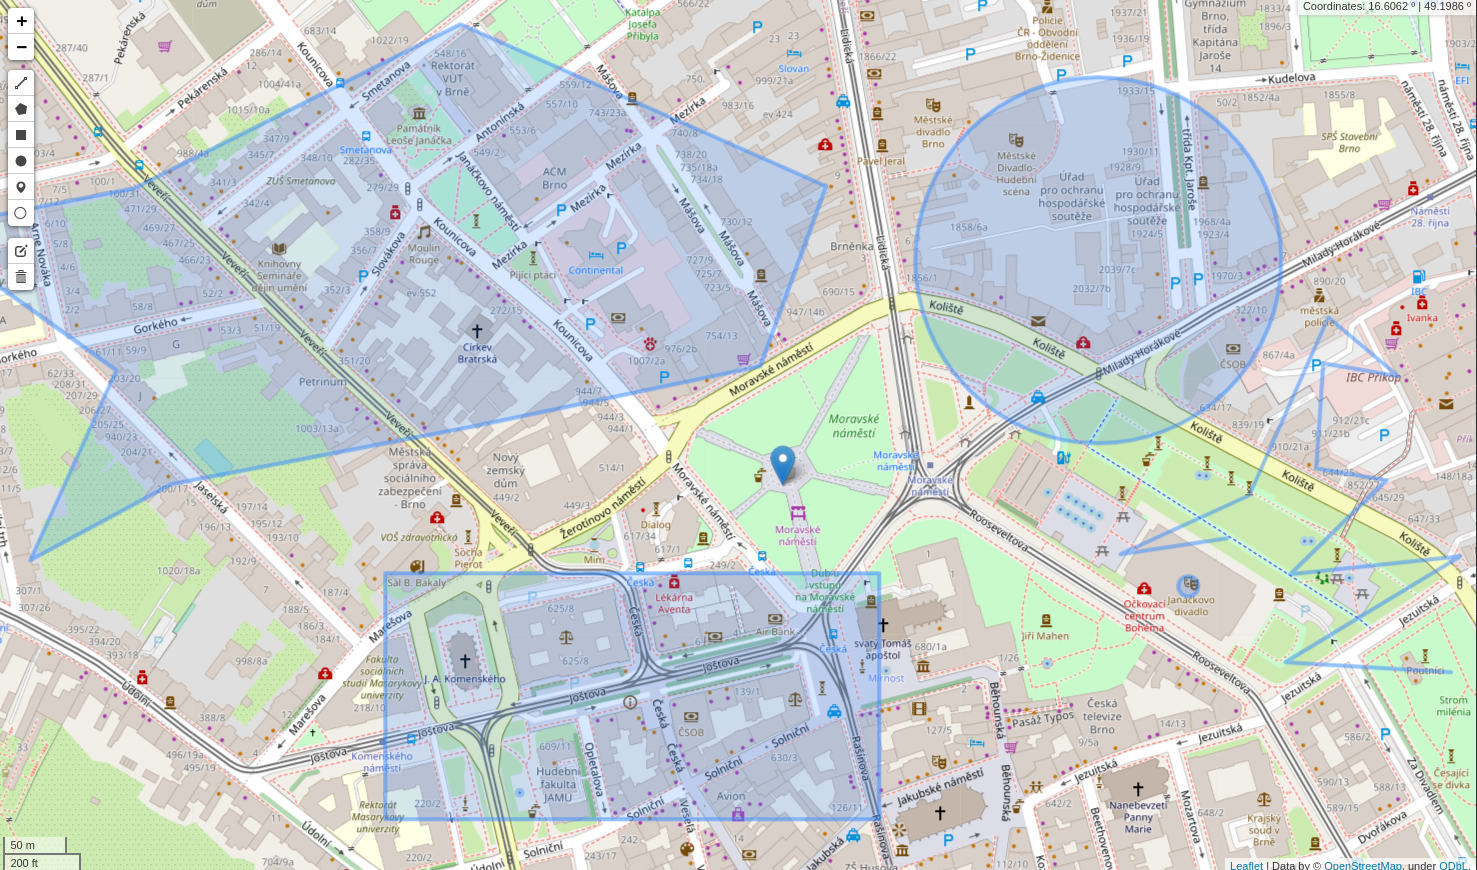
\includegraphics[width=0.8\textwidth]{obrazky-figures/leaflet-draw-screenshot.png}
    \caption{\textbf{Rozšírenie Leaflet.draw} pridáva možnosť kreslenia geometrických útvarov na~mapu \-- krivky, polygóny, obdĺžniky, kruhy, značky a~kruhové značky. Okrem toho je možné pomocou tohto rozšírenia upravovať, presúvať a vymazávať geometrické útvary.}
    \label{fig:leafletdraw}
\end{figure}

\section{HTML}
Jazyk HTML\footnote{HyperText Markup Language, v preklade \emph{Hypertextový značkovací jazyk}.} je jazyk určený na vytváranie webových stránok. Ako už názov napovedá, slovo \emph{hypertextový} naznačuje možnosť odkazov jednotlivých stránok na ostatné. Slovo \emph{značkovací} v spojitosti s jazykmi predstavuje jazyky, ktoré doplňujú text o tzv. \emph{značky} resp.~\emph{tagy}. Všetky značky majú svoje atribúty, ktoré upresňujú jej parametre. Jednotlivé značky je možné do seba vnárať a~spolu tak vytvárajú hierarchickú štruktúru~\cite{kosek1998html}.


\section{CSS}
Štruktúru webových stránok je možné vytvoriť použitím len jazyka HTML, ale na to, aby stránky vyzerali užívateľsky prívetivo, je nutné použiť aj iné nástroje, ktoré pôsobia na~užívateľa prívetivejším dojmom. Preto vznikol mechanizmus \emph{CSS}\footnotetext{Cascading Style Sheets} na vizuálne formátovanie webových stránok. Tento mechanizmus slúži na popis kaskádových štýlov HTML dokumentu.


\section{JQuery}
JQuery\footnote{\url{https://jquery.com}} je rýchla a cross-browser\footnote{Cross-browser kompatibilita je schopnosť webových stránok fungovať v rôznych prehliadačoch.} knižnica z jazyka JavaScript. Zjednodušuje prechádzanie dokumentov HTML, výber DOM\footnote{Document Object Model} elementov, kontrolu udalostí alebo aj vytváranie animácií. Výhodou tejto knižnice je, že je jednoduchou knižnicou na vývoj webových aplikácií. Oproti iným knižniciam v JavaScripte nevyžaduje lepšiu skúsenosť s jazykom JavaScript. Táto knižnica umožňuje okrem už zmienených možností, jednoduchšiu obsluhu \texttt{AJAX} volaní.


\section{AJAX}
Technológia AJAX\footnote{Asynchronous JavaScript and XML} umožňuje meniť obsah stránok bez potreby kompletného načítania zo~servera. Keďže protokol HTTP je bezstavový, akékoľvek stavové informácie je nutné posielať pri každom požiadavku servera a opačne. AJAX nám umožňuje sa takémuto postupu vyhnúť~\cite{lacko2008ajax}. Ako je možné poznať z názvu, AJAX je kombinácia viacerých prvkov:
\begin{itemize}
    \item HTML a CSS na prezentovanie informácií,
    \item DOM na zobrazenie prezentovaných informácií,
    \item metóda na výmenu dát medzi prehliadačom a serverom (napr. XMLHttpRequest objekt),
    \item formát dát posielaný medzi prehliadačom a serverom (napr. XML)
\end{itemize}

V mojej aplikácií som použil AJAX technológiu na aktualizáciu súradníc pri zmene veľkosti alebo presune oblasti určenej na vytvorenie heat mapy.


\section{Bootstrap}
Bootstrap je sada nástrojov, ktorá obsahuje rozšírenie pre jazyky HTML, CSS a JavaScript. Umožňuje vytvárať pomocou veľkého množstva rôznorodých komponentov interaktívne webové stránky. Vyžaduje určitú znalosť HTML a~CSS, pretože väčšinu komponentov je možné vkladať iba pomocou HTML a CSS~\cite{bootstrap}.

V mojej aplikácií používam tzv. \emph{Alert} komponentu t.j. výstražnú správu. Ak sa nepodarila vytvoriť heat mapa z~parametrov poslaných na server, server pošle správu užívateľovi, že heat mapa sa pre zadanú oblasť nepodarila vytvoriť.



\chapter{Návrh}
\label{navrh}
V tejto kapitole je popísaný návrh systému, na ktorom je založená celá aplikácia. Na začiatku tejto kapitoly sa analyzujú požiadavky na aplikáciu a popisujú kľúčové vlastnosti, ktoré musia byť splnené. Táto kapitola zahŕňa aj bližšie popísanie použitých technológií a~dôvody, prečo boli zvolené dané technológie pri návrhu aplikácie.


\section{Analýza požiadavkov}
\label{sec:analysis}
Požiadavky sú potrebné pri akomkoľvek návrhu aplikácie. S požiadavkami sa treba zamyslieť, ako sa dajú navrhnúť a implementovať. Primárnym cieľom tejto bakalárskej práce je vytvoriť aplikáciu, ktorá na základe získaných dát vytvorí odhady pravdepodobnosti výskytu osôb. Túto aplikáciu je možné vytvoriť tak, aby ju bolo možné v budúcnosti rozšíriť o viaceré funkcionality, ale aj aby bola užívateľsky prívetivá.

\subsection{Vstupné dáta}
Prvou požiadavkou pri vytvorení aplikácie je spracovanie vstupných dát získaných od užívateľa.
Vstupné dáta je možné rozdeliť na dva typy: súradnice a~hodnoty pravdepodobností.

\subsubsection{Súradnice}
Prvým typom vstupných dát sú súradnice, ktoré užívateľ bude môcť zadať rôznymi spôsobmi. Spôsoby získavania vstupných súradníc budú inšpirované získavaním hraničných súradníc na~stránke projektu OpenStreetMap.

Jednou z možností je využitie knižnice \texttt{Leaflet.draw}. Užívateľ v navrhovanej aplikácií by mal byť schopný vykresliť na mapu plochu, z~ktorej by chcel zistiť, aká je pravdepodobnosť výskytu osôb v~danej oblasti. Z~tejto nakreslenej plochy sa dá zistiť, aké sú hranice danej plochy, t.j. aká je minimálna a~maximálna hodnota zemepisnej dĺžky a~aká je minimálna a~maximálna hodnota zemepisnej šírky nakreslenej plochy. Tento spôsob získavania vstupných dát je zobrazený na obrázku~\ref{fig:osm-export}.

Druhá možnosť získavania vstupných súradníc, takisto používaná na stránke projektu OpenStreetMap, by mohla fungovať na základe získavania hraníc mapy, ktorá je na stránke zobrazená. To znamená, že horná a dolná hranica mapy predstavujú zemepisné dĺžky, ľavá a pravá hranica mapy predstavujú zemepisné šírky.

Tretiu možnosť získavania vstupných súradníc je možné použiť v kombinácií s~už zmienenými možnosťami. Užívateľ by mal byť schopný zadať všetky štyri hraničné súradnice manuálne. Pri návrhu takejto možnosti je potrebné myslieť na~to, že súradnica hornej (severnej) hranice musí byť väčšia ako súradnica dolnej (južnej) hranice a súradnica pravej (východnej) hranice musí byť väčšia ako súradnica ľavej (západnej) hranice.

\begin{figure}[ht]
    \centering
    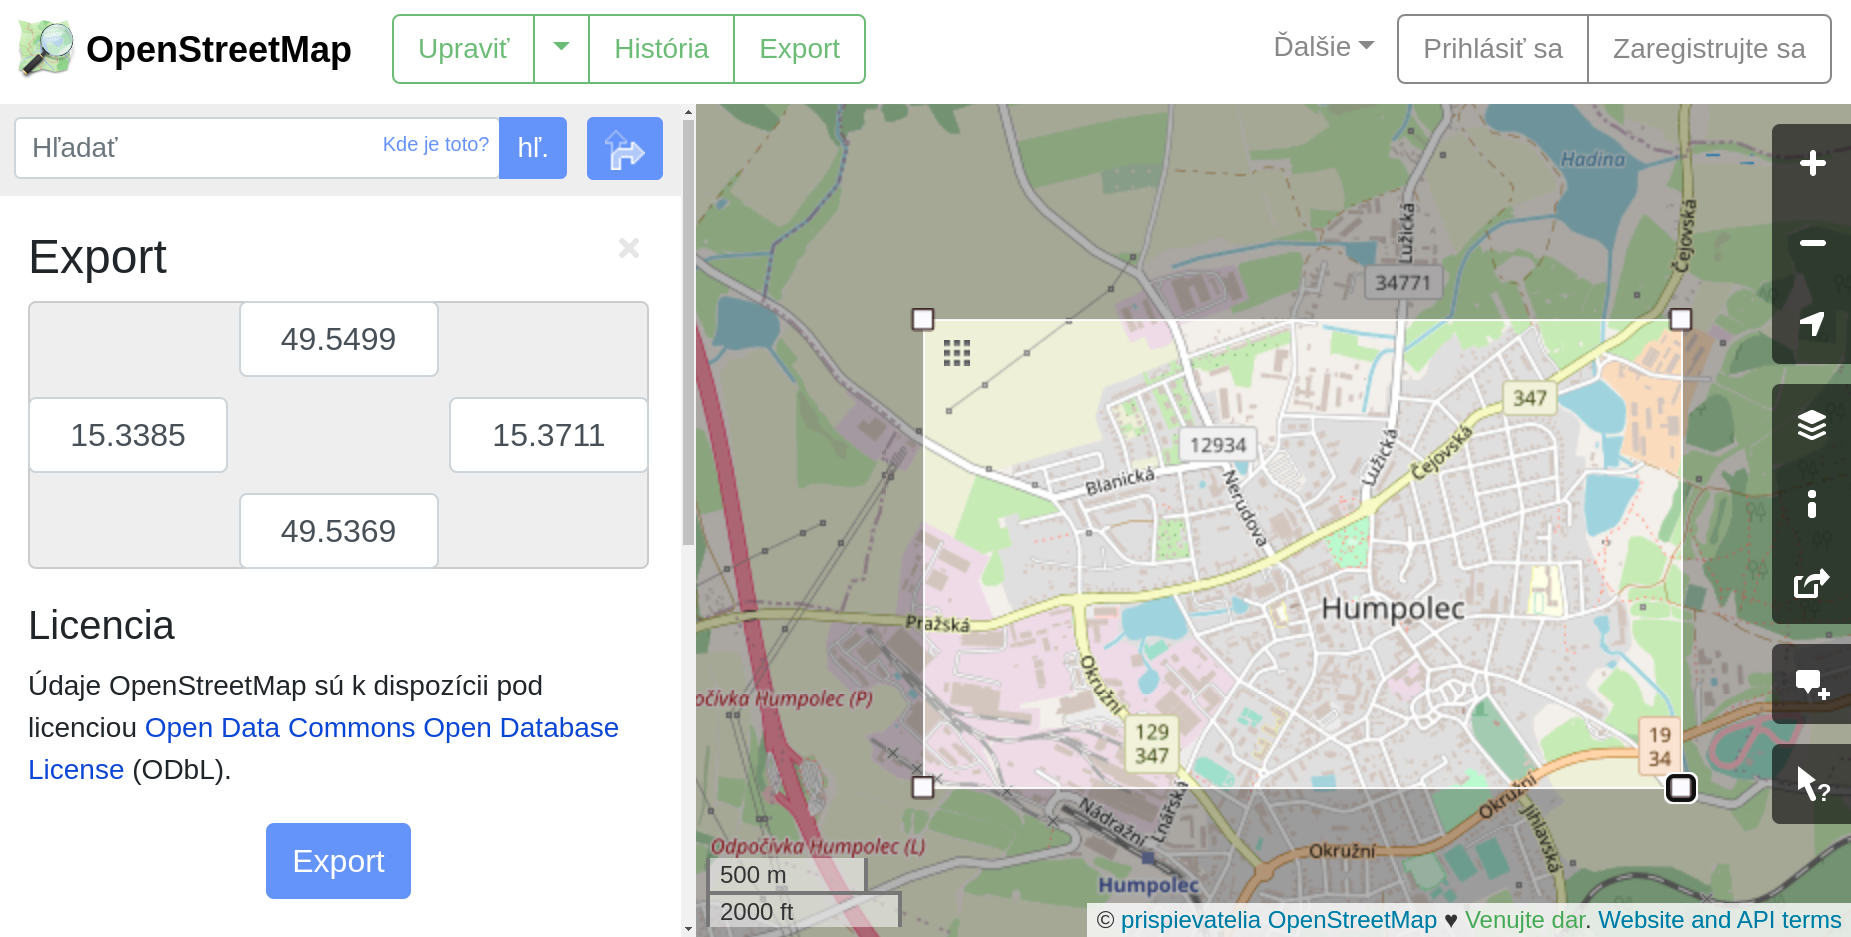
\includegraphics[width=0.8\textwidth]{obrazky-figures/openstreetmap-export.png}
    \caption{Export dát na stránke projektu OpenStreetMap}
    \label{fig:osm-export}
\end{figure}
    
\subsubsection{Hodnoty pravdepodobností}
Druhým typom vstupných dát od užívateľa sú hodnoty pravdepodobností resp.~intenzít pre~značky. Vo~väčšine prípadoch počet týchto vstupných hodnôt pravdepodobností môže byť aj viac ako 100, preto vhodným návrhom pre zadávanie hodnôt je použitie externého súboru. V tomto súbore by mal užívateľ mať možnosť zadefinovať, ktoré značky by sa mali použiť pri vykresľovaní heat vrstvy a aké hodnoty pravdepodobností by mali mať tieto značky.

\subsection{Zobrazovanie heat vrstvy}
Získané hodnoty pravdepodobností značiek by mali byť pre užívateľa informatívne a užívateľ by mal byť schopný vidieť z danej oblasti, aká je pravdepodobnosť výskytu osôb v danej oblasti. Vhodnou voľbou pre zobrazovanie pravdepodobností by bolo vytvorenie heat vrstvy na~mape, ktorá bude interpretovať hodnoty pravdepodobností v~danej oblasti.

Hodnoty pravdepodobností je možné interpretovať základnými farebnými schémami. Celé farebné spektrum sa skladá z kombinácií troch farieb (červená, zelená a modrá). Teplé farby sa väčšinou spájajú s ohňom a slnkom, preto sem patria farby ako červená, oranžová a žltá. Keď si ale predstavíme zasnežené hory, farebná škála sa ihneď zmení na studenú, kde prevládajú farby ako modrá, zelená a fialová. V navrhovanej aplikácii by sa dali využiť tieto farebné odtiene na zobrazovanie pravdepodobností. V oblastiach s~väčšou pravdepodobnosťou výskytu osôb by aplikácia mala zobrazovať teplejšie farby a~na~druhej strane v~oblastiach s~menšou pravdepodobnosťou by aplikácia mala zobrazovať studenšie farby. V~oblastiach, kde sú hodnoty pravdepodobností pre dané značky rovné $0$ by nemala byť na~mapu vykreslená v~danej oblasti heat vrstva.


\section{Architektúra}
Cieľom bakalárskej práce je vytvorenie aplikácie, ktorá odhadne pravdepodobnosť výskytu osôb v~danej oblasti. Pomocou získaných požiadavkov na aplikáciu je možné vytvoriť architektúru danej aplikácie. Aplikácia bude musieť vedieť získavať hraničné súradnice z~oblasti, ktorú vyberie užívateľ. Horná a~spodná hranica  danej oblasti budú reprezentovať zemepisnú dĺžku, ľavá a~pravá hranica budú reprezentovať zemepisnú šírku. V rámci modifikácie objektov by mal byť užívateľ schopný upravovať tvar nakreslených obdĺžnikov. Pri zmenení veľkosti obdĺžnika alebo presunutia obdĺžnika na inú časť mapy by mala aplikácia zareagovať a~zobraziť tieto upravené hodnoty súradníc v~grafickom užívateľskom rozhraní. Tieto štyri súradnice by mala aplikácia použiť na~získanie dát o~geografických objektoch (bodoch, čiarach a~polygónoch). Získané geografické objekty by malo byť možné použiť pri vytváraní heat bodov na~vytvorenie heat vrstvy. 


\section{Dátový model}
Dátový model reprezentuje dáta, s ktorými bude aplikácia pracovať. Dáta, ktoré je možné získať pri spracovávaní mapových dát, sú geografické objekty. Informácie o získaných geografických objektoch a~ich priradenie ku značkám na mape bude aplikácia uchovávať vo~svojej pamäti vo~forme dátových rámcoch.

\subsubsection{Dátový rámec}
Dátový rámec je dvoj-dimenzionálna dátová štruktúra, podobná tabuľke s~riadkami a~stĺpcami. Každý riadok dátového rámca reprezentuje jeden geografický objekt. Definícia geometrického objektu sa bude nachádzať v~stĺpci \emph{geometry}. Okrem definície geografického objektu sa v~tomto riadku bude nachádzať aj~akú značku na~mape predstavuje daný geografický objekt. 

\subsubsection{Geografický objekt}
Geografický objekt, ktorý sa bude nachádzať v stĺpci \emph{geometry} dátového rámca, môže byť jedným z~hodnôt: \emph{Point}, \emph{LineString} alebo \emph{Polygon}. Tieto typy predstavujú základné geometrické objekty. Typy, ktoré rozširujú tieto základné typy, sú rozšírenými geometrickými objektami. Sú od nich rozlíšené predponou \textbf{Multi}, t.j. \emph{MultiPoint}, \emph{MultiLineString} a~\emph{MultiPolygon}. Formát súradníc závisí od typu geografického objektu.

\begin{itemize}
\item \textbf{Point} predstavuje pole dvoch číselných hodnôt, ktoré reprezentujú x-ovú a y-ovú súradnicu (viď.~\ref{lst:point}).

\lstset{
    caption={Príklad súradníc typu \emph{Point}.},
    label={lst:point},
    basicstyle=\ttfamily\normalsize\bfseries,
    xleftmargin=.28\textwidth, xrightmargin=.28\textwidth
}
\begin{lstlisting}
coordinates: [40.3, 29.8]
\end{lstlisting}

\item \textbf{LineString} predstavuje pole bodov, kde prvý bod je začiatočným bodom a~posledný bod je koncovým bodom čiary (viď.~\ref{lst:linestring}).

\lstset{
    caption={Príklad súradníc typu \emph{LineString}.},
    label={lst:linestring},
    basicstyle=\ttfamily\normalsize\bfseries,
    xleftmargin=.2\textwidth, xrightmargin=.2\textwidth
}
\begin{lstlisting}
coordinates: [[20.5, 30.1], [21.8, 31.0]]
\end{lstlisting}

\item \textbf{Polygon} predstavuje pole bodov, ako u~typu \emph{LineString} s~tým rozdielom, že body sú pospájané do~mnohouholníka. Prvý bod tohto objektu musí byť aj koncovým bodom. Vo~výpise~\ref{lst:polygon} je možné vidieť, ako je potrebné zadefinovať trojuholník.

\lstset{
    caption={Príklad súradníc typu \emph{Polygon}.},
    label={lst:polygon},
    basicstyle=\ttfamily\normalsize\bfseries,
    xleftmargin=.02\textwidth, xrightmargin=.05\textwidth
}
\begin{lstlisting}
coordinates: [[20.0, 20.0], [21.9, 21.9], [20.0, 22.8], [20.0, 20.0]]
\end{lstlisting}
\end{itemize}


\section{Štruktúra systému}
Pri tvorbe návrhu sa vychádzalo z~analýzy požiadavkov v sekcii~\ref{sec:analysis}. Pri zadávaní vstupných súradníc sa bude môcť užívateľ rozhodnúť, či chce na mapu nakresliť obdĺžnik, z ktorého bude vytvorená heat vrstva na mape alebo či zadá hraničné súradnice textového poľa. Ak užívateľ nakreslí na mapu obdĺžnik (resp. zobrazí si na mape určitú časť), systém spracuje tento nakreslený objekt na mape a použitím asynchrónnej správy zobrazí tieto súradnice vo~formulári, kde ich bude môcť užívateľ prípadne upraviť. Takúto úpravu by mal užívateľ byť schopný vykonať veľakrát. Takisto by mohol užívateľ upravovať veľkosť aj~pozíciu nakresleného obdĺžnika. Okrem toho by mohol užívateľ odstraňovať nakreslenú plochu. Ak budú zadané súradnice od užívateľa, tak potom by bolo možné vytvoriť heat vrstvu. Užívateľ jednoducho bude môcť poslať požiadavok na server, kde sa spracuje tento požiadavok a~server pošle užívateľovi po určitej dobe trvania mapu s vytvorenou heat vrstvou. Všeobecnejší návrh, ako by mohla aplikácia fungovať, je zobrazený na obrázku~\ref{fig:navrh-diagram}.

\begin{figure}[h]
    \centering
    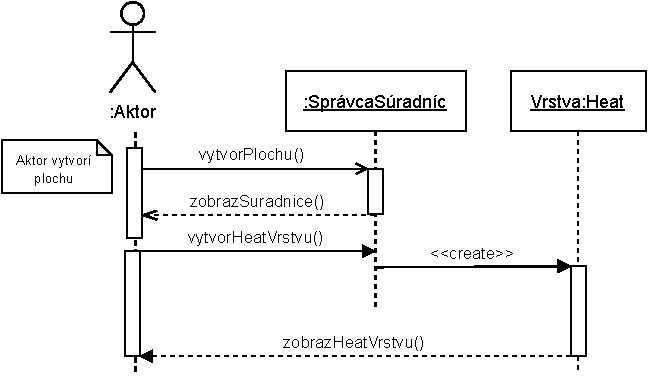
\includegraphics[width=0.9\linewidth]{obrazky-figures/seq-diagram.pdf}
    \caption{Sekvenčný diagram, ktorý zobrazuje, v akom poradí budú vykonávané jednotlivé operácie.}
    \label{fig:navrh-diagram}
\end{figure}

Aby systém fungoval správne, bude potrebné brať vstupné údaje o pravdepodobnostiach. Tieto pravdepodobnosti ale užívateľ nebude môcť zadať v užívateľskom grafickom rozhraní. Keďže každá značka má definované, aké môže mať kľúče s~hodnotami (\texttt{key=value}), bude potrebné pre~každú takúto dvojicu hodnôt priradiť hodnoty, ktoré budú vytvárať heat vrstvu. 


% \todo{TODO}
% \blindtext[2]

% \Blindtext


% \chapter{Implementácia}
% \label{implementacia}
% \todo{TODO}

% \blindtext[13]


% \chapter{Testovanie}
% \label{testovanie}
% \todo{TODO}

% \blindtext[1]

% \blindtext[10]



% \chapter{Záver}
% \label{zaver}
% \todo{TODO}

% \blindtext[3]
